\section{Understanding the Challenge}\label{ch:challenge}\raggedbottom
blablabla \ldots
As we continue with Sections \ref{sec:prob} and \ref{sec:eval}, we will 
rely on \cite{higgsPaper}, as this paper describes these points from the challenge-creators point of view.

\subsection{The Data}
\subsection{The data}\label{sec:data}
All data provided by the challenge and the opendata.cern dataset \cite{higgsData} was created by the official ATLAS full detector simulator in a two-part process. The simulator first produces proton-proton collisions, called \emph{events}. Then it tracks these via a virtual model of the ATLAS-detector. The resulting data emulates the statistical properties of the real events. By this procedure it is possible to exactly know, if an event is a searched \emph{signal}, or \emph{background}. Signal-events are generated by previously mentioned \emph{tau tau decay of the Higgs Boson} ($\mathrm{H}\rightarrow\tau\tau $). Background-events originate from three known processes\footnote{These processes are decay of Z bosons, W bosons and pairs of top quarks. There are more processes known that resemble ($\mathrm{H}\rightarrow\tau\tau $), for simplicity only these three are used as background for this challenge \cite{higgsPaper}.} which produce radiation similar to the signal \cite{higgsPaper}. The feature \texttt{Label} expresses the true class of an event, "$s$" for signals and "$b$" for background.

Every event has a feature \texttt{Weight}, a result of the simulation. The weights correspond to an estimation of the number of expected events of this class in a \emph{region} during a fixed time interval\cite{higgsPaper}.\\
For instance:
A group of 100 events of both classes, "$s$" and "$b$", originates from the region $A$, for which we expect 90\% of events to be background and 10\% being signal.
For another region $B$, we expect a 50/50 distribution. The weight of an event in a region is directly related to the expected probability of its occurrence. This results in a so-called \emph{importance weighting} and causes the mean of the weights for signal-events to be considerably smaller than for background-weights. We will see, that the challenge evaluation utilizes this to punish incorrectly classifying background as signal.

The features \texttt{Weight} and \texttt{Label} were originally only provided in the training dataset. The data used in this thesis is expanded by complete \texttt{Weight}-, \texttt{Label}-features and the Kaggle-specific features \texttt{KaggleSet} and \texttt{KaggleWeight}. The last one is a normalization of \texttt{Weight} for the total number of signal- or background-events with the same \texttt{KaggleSet} feature.
This information enables us to recreate the original datasets using the opendata.cern dataset.

The physical features are separated in two types. Features containing so-called primitive data, properties of events explicitly measured by the simulated ATLAS detector, use the prefix "\texttt{PRI\_}" in their names. The second type is called derived data, which are features that have been computed from primitive features. Their labels use the prefix "\texttt{DER\_}".\\
Tab. \ref{tab:data} is a complete data vector retrieved from \cite{higgsData}.

\begin{table}
\begin{center}
	\begin{tabular}{|l|r|}
		\hline
		Feature name & Feature value \\
		\hline
		\texttt{EventId} & 100000 \\
		\hline
		\texttt{DER\_mass\_MMC} & 138.47 \\
		\hline
		\texttt{DER\_mass\_transverse\_met\_lep} & 51.655 \\
		\hline
		\texttt{DER\_mass\_vis} & 97.827 \\
		\hline
		\texttt{DER\_pt\_h} & 27.98 \\
		\hline
		\texttt{DER\_deltaeta\_jet\_jet} & 0.91 \\
		\hline
		\texttt{DER\_mass\_jet\_jet} & 124.711 \\
		\hline
		\texttt{DER\_prodeta\_jet\_jet} & 2.666 \\
		\hline
		\texttt{DER\_deltar\_tau\_lep} & 3.064 \\
		\hline
		\texttt{DER\_pt\_tot} & 41.928 \\
		\hline
		\texttt{DER\_sum\_pt} & 197.76 \\
		\hline
		\texttt{DER\_pt\_ratio\_lep\_tau} & 1.582 \\
		\hline
		\texttt{DER\_met\_phi\_centrality} & 1.396 \\
		\hline
		\texttt{DER\_lep\_eta\_centrality} & 0.2 \\
		\hline
		\texttt{PRI\_tau\_pt} & 32.638 \\
		\hline
		\texttt{PRI\_tau\_eta} & 1.017 \\
		\hline
		\texttt{PRI\_tau\_phi} & 0.381 \\
		\hline
		\texttt{PRI\_lep\_pt} & 51.626 \\
		\hline
		\texttt{PRI\_lep\_eta} & 2.273 \\
		\hline
		\texttt{PRI\_lep\_phi} & -2.414 \\
		\hline
		\texttt{PRI\_met} & 16.824 \\
		\hline
		\texttt{PRI\_met\_phi} & -0.277 \\
		\hline
		\texttt{PRI\_met\_sumet} & 258.733 \\
		\hline
		\texttt{PRI\_jet\_num} & 2 \\
		\hline
		\texttt{PRI\_jet\_leading\_pt} & 67.435 \\
		\hline
		\texttt{PRI\_jet\_leading\_eta} & 2.15 \\
		\hline
		\texttt{PRI\_jet\_leading\_phi} & 0.444 \\
		\hline
		\texttt{PRI\_jet\_subleading\_pt} & 46.062 \\
		\hline
		\texttt{PRI\_jet\_subleading\_eta} & 1.24 \\
		\hline
		\texttt{PRI\_jet\_subleading\_phi} & -2.475 \\
		\hline
		\texttt{PRI\_jet\_all\_pt} & 113.497 \\
		\hline
		\texttt{Weight} & 0.00081448039868 \\
		\hline
		\texttt{Label} & s \\
		\hline
		\texttt{KaggleSet} & t \\
		\hline
		\texttt{KaggleWeight} & 0.00265331133733 \\
		\hline	
	\end{tabular}
\end{center}
\caption{Event 100000 provided by opendata.cern data\cite{higgsData}}
\label{tab:data}
\end{table}

One might expect decent knowledge in physics as key in succeeding in the challenge. However, the top participants did not use a lot domain knowledge for feature or method selection. One goal of the challenge was to set a task for data scientists without any background in physics \cite{higgsPaper}.

\subsubsection{Data visualization}
To get first information about our data we use basic methods of data analysis.
To evaluate single features for classification we plot a histogram of the class labels' distribution in Fig. \ref{fig:hist1}. A useful way to learn about relations between features is to create \emph{scatter plots} of all two-features combinations, see Fig. \ref{fig:scat1}.
Using these visualizations, we can identify features with good properties for our task.

%More details about specific features of the dataset can be found in Appendix \ref{app:data}.

\begin{figure}
\centering
\begin{minipage}[t]{.49\textwidth}
  \centering
  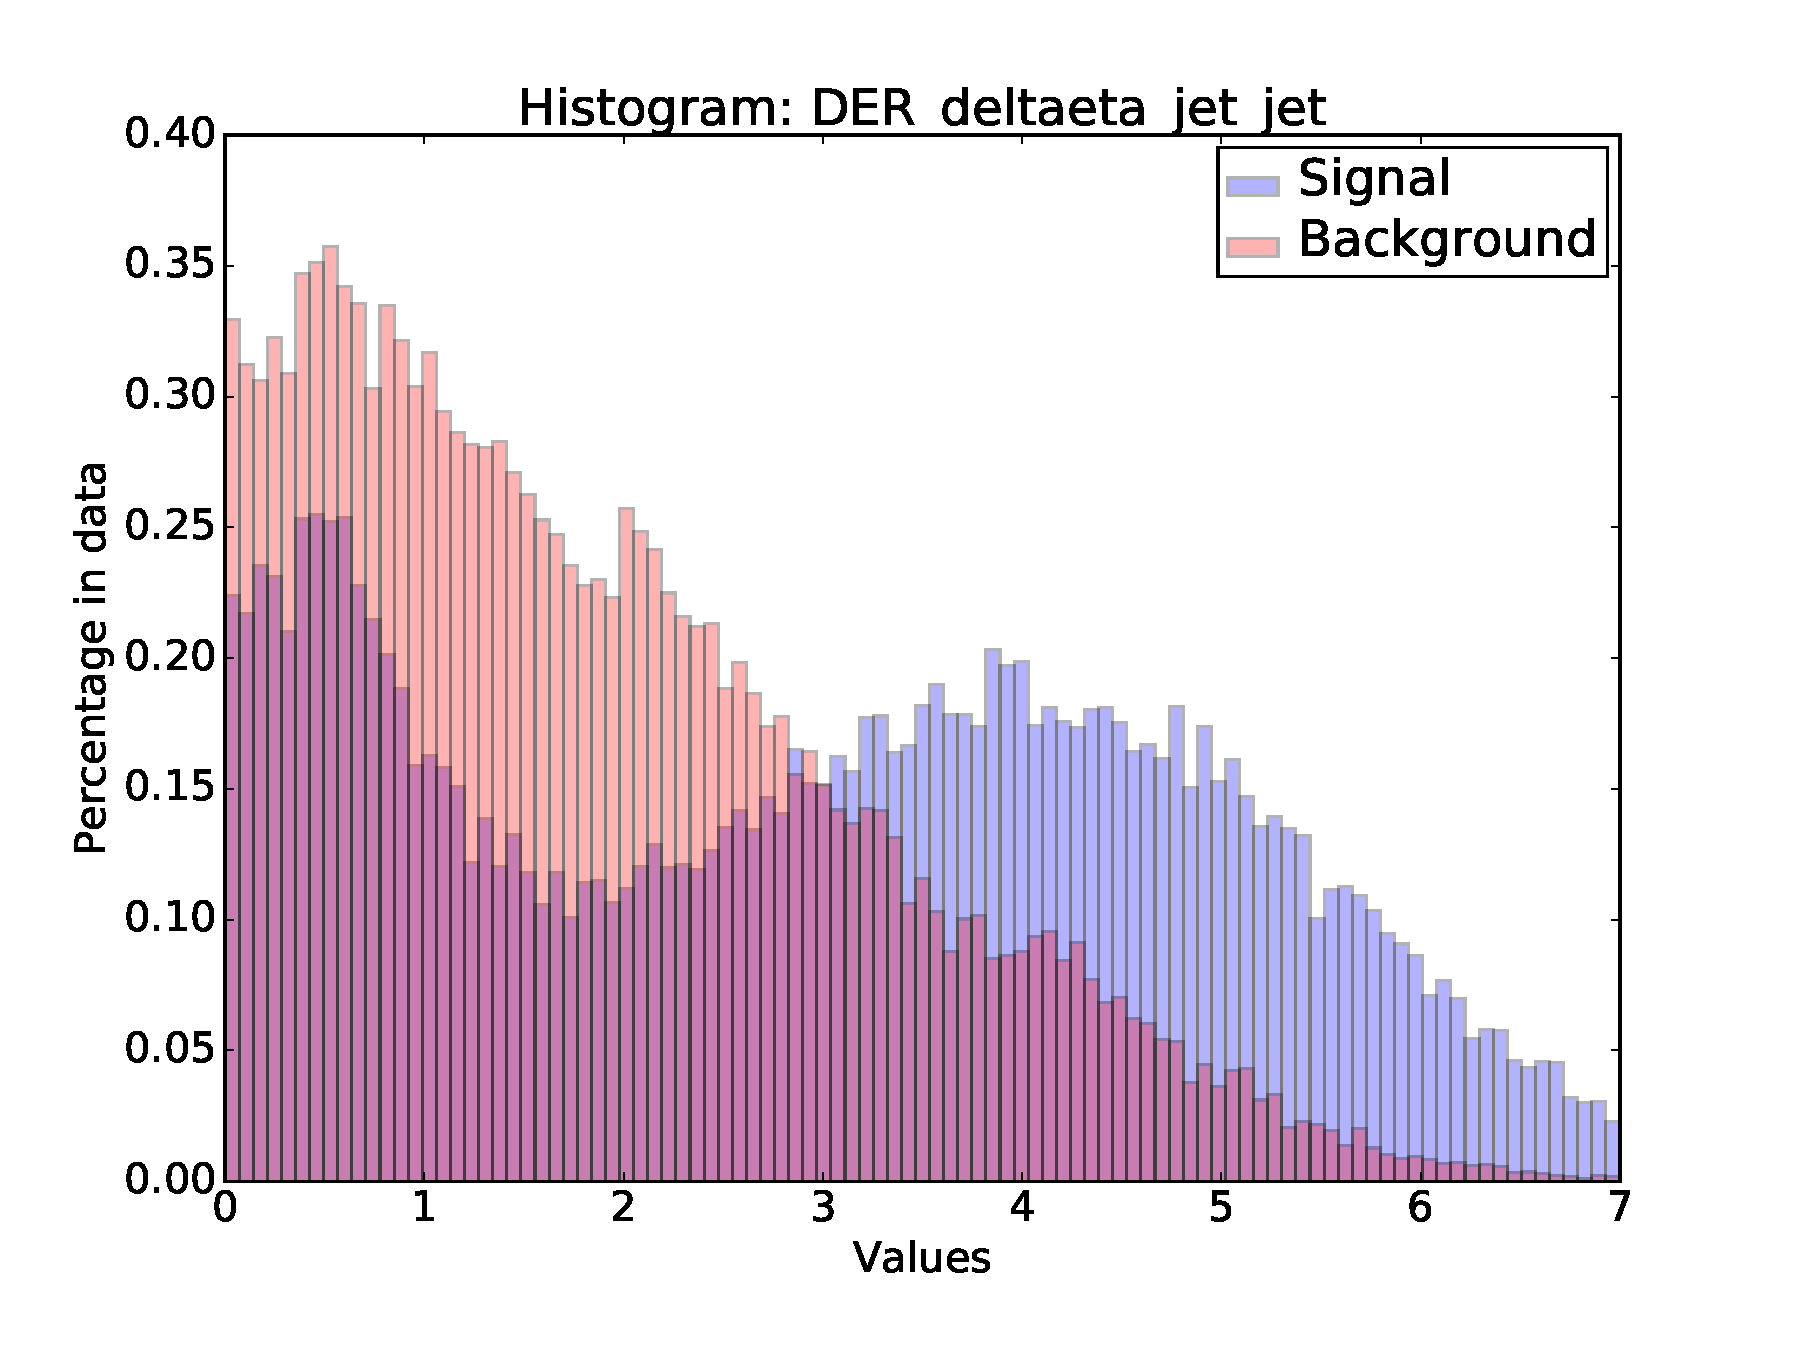
\includegraphics[width=\linewidth]{images/histogram.pdf}
  \captionof{figure}{Histogram of \emph{DER\_deltaeta\_jet\_jet}}
  \label{fig:hist1}
\end{minipage}%
\hspace{0.5em}
\begin{minipage}[t]{.49\textwidth}
  \centering
  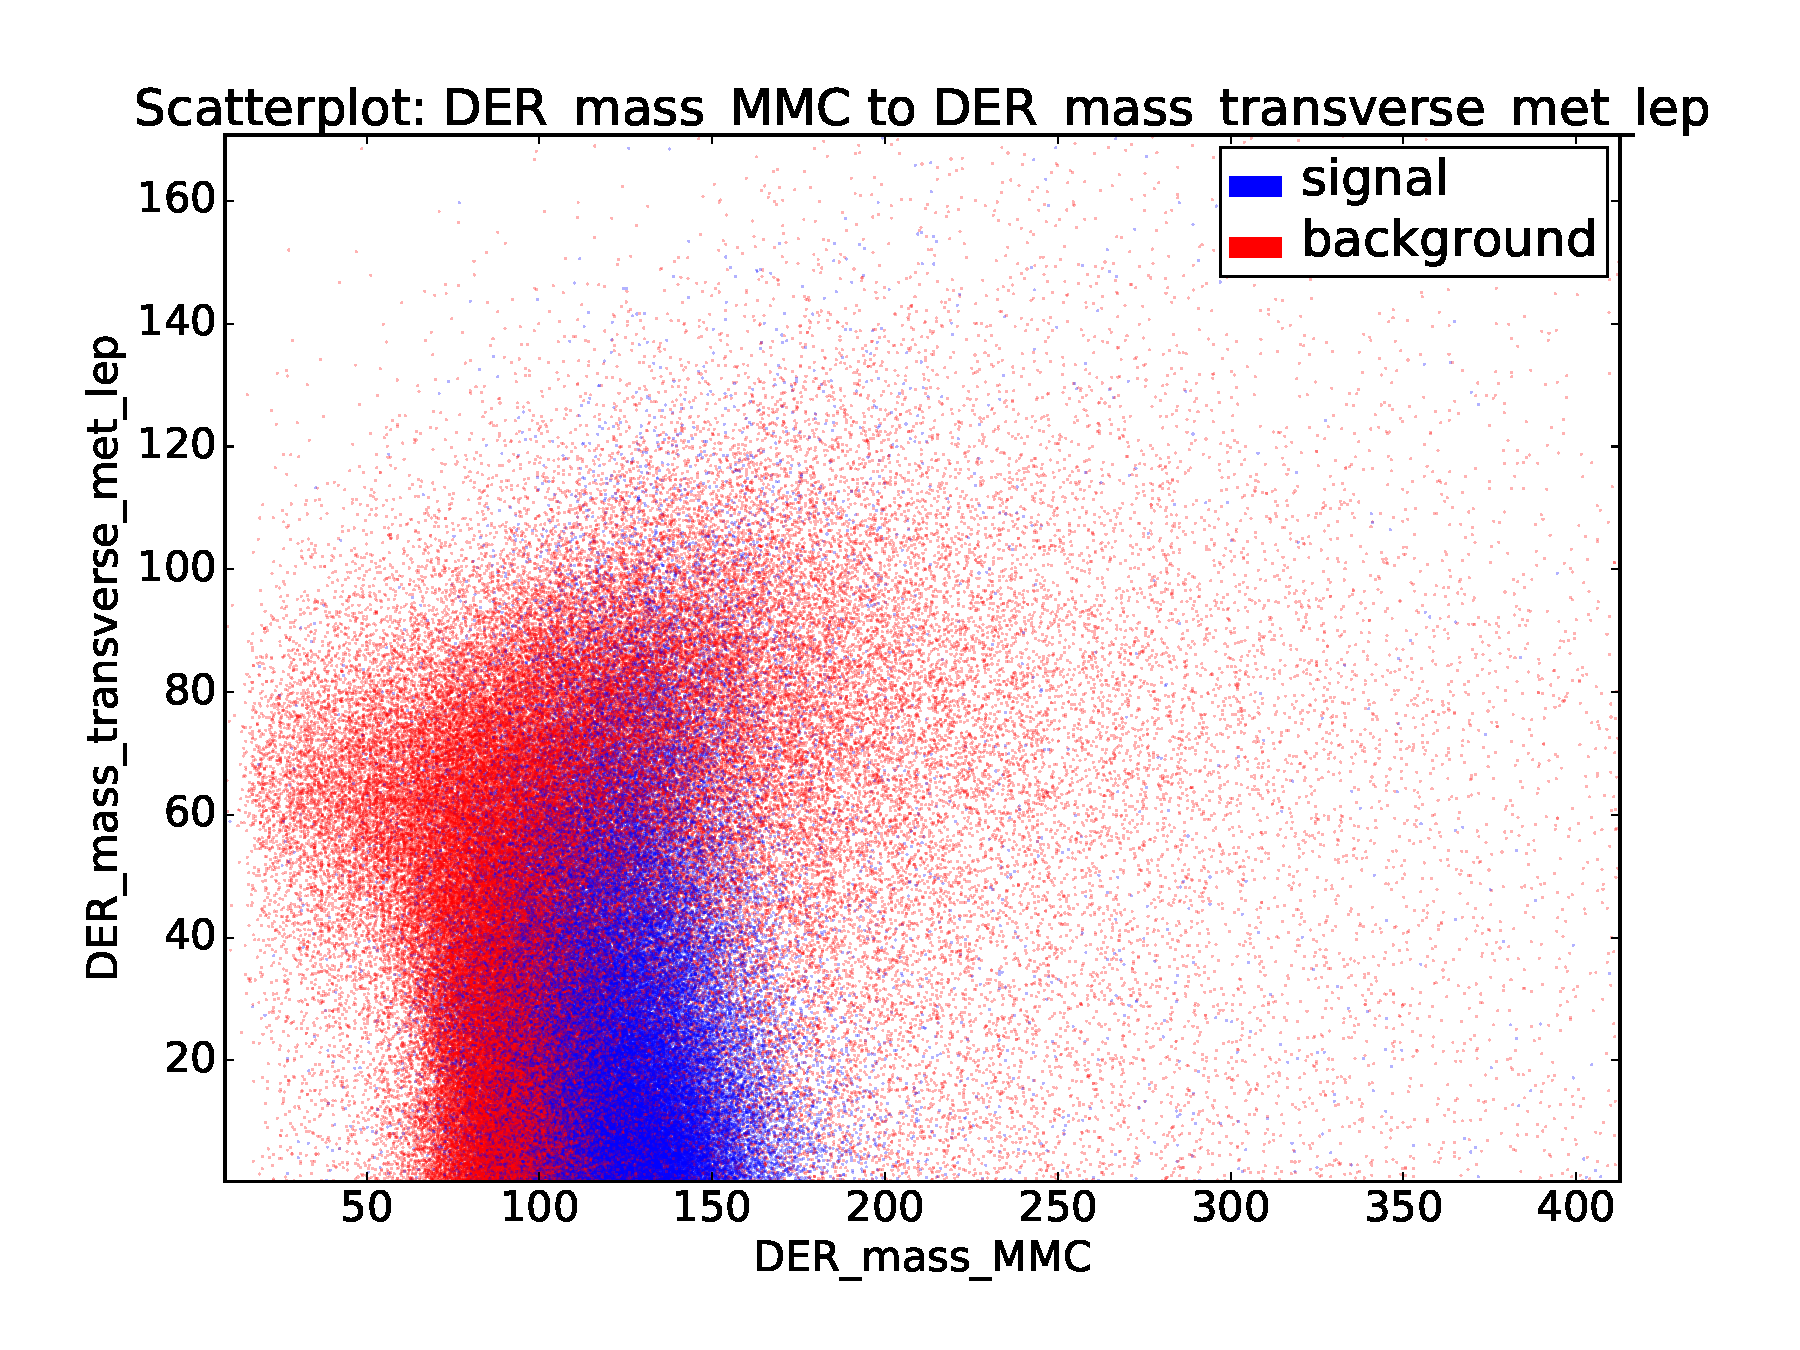
\includegraphics[width=\linewidth]{images/scatter.png}
  \captionof{figure}{Scatter plot of \emph{DER\_mass\_MMC} to \emph{DER\_mass\_transverse\_met\_lep}}
  \label{fig:scat1}
\end{minipage}
\end{figure}


\subsection{The formal problem}\label{sec:prob}
\subsection{The classification problem}\label{sec:prob}
We use the formal description of the challenge as in \cite{higgsPaper}.\\
Let $D = {(x_i,y_i,w_i)}, \ i \ \epsilon \ \{1,\ldots,n\}$ be the training sample with $n$ events, where:

\begin{itemize}
	\item $x_i \ \epsilon \ \mathbb{R}^{d}$ is a $d$-dimensional vector
	\item $y_i \ \epsilon$ \{b,s\} is the label
	\item and $w_i \ \epsilon \ \mathbb{R}^{+}$ is a non-negative weight.
\end{itemize}

The sum of signal weights
$$S = \sum_{y_i = s} w_i$$
and the sum of background weights
$$B = \sum_{y_i = b} w_i$$
represent the \emph{expected total number} of signal and background events, during the time of actual data recording.

Let a function $$g: \mathbb{R}^{d} \rightarrow \{b,s\}$$
be a binary classifier.
The set $$G_s = \{x : g(x) = s \}$$ is called the \emph{selection region}.

Our task is to find a function \emph{g} that maximizes the AMS, that we introduce in the next section.\\
For a given classifier \emph{g} we maintain an \emph{index set} 
$ \hat{G}_s = \{i : g(x_i) = s \} $ of training points that $g$ classifies as signal and an \emph{index set} $ \hat{G}_b = \{i : g(x_i) \neq s \} $. By definition each point can only be one index set, i.e. ($\hat{G}_s \cap \hat{G}_b = \emptyset$).

The index set can be turned into a submission file for the challenge, but requires to fit the following format.

\begin{verbatim}
EventId,RankOrder,Class
350000,2,b
350001,54493,s
...
899999,32455,b
\end{verbatim}

All events must have a prediction \texttt{b} or \texttt{s}. \texttt{RankOrder} shall state the probability of an event being the signal \texttt{s}, compared to all other events, e.g. rank \texttt{550000} is being considered as the most signal-like event. However, predicting the right event ranking was not necessary for the challenge.


\subsection{The evaluation}\label{sec:eval}
The evaluation of a single submission to the challenge is related to the common practice in particle physics to rate a discovery by its statistical significance, in this case 

%hier evtl mehr über die Entstehung?

\begin{equation}\label{eq:Z}
	Z = \sqrt{2 \left(n \ln{\left( \frac{n}{\mu_b} \right)} -
	n + \mu_b \right)}
\end{equation}

where $n$ is the total number of observed events and $\mu_b$ is the expected number of background-events.\\
Often in particle physics a significance of at least Z=5 (a five-sigma effect) is regarded as sufficient to claim a discovery \cite{higgsPaper}.

By estimating $n=s+b$ and $mu_b = b$ in Eq. \eqref{eq:Z}, we get the $Approximate$ $Median$ $Significance$ (AMS)

\begin{equation}\label{eq:AMS_1}
	AMS = \sqrt{2 \left( \left( s+b \right) \ln{ \left(1+ \frac{s}
	{b}  \right)} - s \right)}
\end{equation}

which is used by high-energy physicists for optimizing the selection region for stronger discovery significance \cite{higgsPaper}. 

For the challenge, a regularization-term $b_{reg}$ was introduced as an artificial shift to $b$ to decrease variance of the AMS, as this makes it easier to compare the participants if the optimal signal region was small. "The value $b_{reg}=10$ was determined using preliminary experiments." \cite{higgsPaper}

This addition to Eq. \eqref{eq:AMS_1} makes the final evaluation-formula complete:

\begin{equation}\label{eq:AMS_2}
	AMS_2 = \sqrt{2 \left( \left( s+b+b_{reg} \right) \ln{ \left(1+ \frac{s}
	{b+b_{reg}}  \right)} - s \right)}
\end{equation}

For simplicity, we will call it just AMS, as Eq. \eqref{eq:AMS_1} will not have further appearances in this thesis.

\subsubsection{The Leaderboards}
%testdata split in private and public set => KaggleSet
%weights are normalized => KaggleWeight
%compare public and private LB (graphic analysis on forums)

\subsubsection{Alternative objective functions}
For classification, a data scientist wants to train a classifier on an \textit{objective function}. Properties of the AMS (like using the logarithm) make it difficult to use it as objective function, some alternatives were proposed by the challenge-creators \cite{higgsPaper} and some challenge-participants via the Kaggle-Forum \cite{higgsForum}

\begin{itemize}
	\item alternative objective function: $ \frac{s}{\sqrt{b}} $
	\begin{itemize}
		\item only valid when $s \ll b \ and \ b \gg 1$
	\end{itemize}
\end{itemize}



\begin{equation}\label{eq:Z}
	Z = \sqrt{q_0} = \sqrt{2 \left(n \ln{\left( \frac{n}{\mu_b} \right)} -
	n + \mu_b \right)}
\end{equation}

\begin{equation}\label{eq:AMS_3}
	\frac{s}{\sqrt{b}}
\end{equation}



\eqref{eq:AMS_2}
\eqref{eq:AMS_3}
\eqref{eq:Z}



%




% Default to the notebook output style


% Inherit from the specified cell style.






    
\documentclass{article}

    
        
    
    \usepackage{graphicx} % Used to insert images
    \usepackage{adjustbox} % Used to constrain images to a maximum size 
    \usepackage{color} % Allow colors to be defined
    \usepackage{enumerate} % Needed for markdown enumerations to work
    \usepackage{geometry} % Used to adjust the document margins
    \usepackage{amsmath} % Equations
    \usepackage{amssymb} % Equations
    \usepackage{eurosym} % defines \euro
    \usepackage[mathletters]{ucs} % Extended unicode (utf-8) support
    \usepackage[utf8x]{inputenc} % Allow utf-8 characters in the tex document
    \usepackage{fancyvrb} % verbatim replacement that allows latex
    \usepackage{grffile} % extends the file name processing of package graphics 
                         % to support a larger range 
    % The hyperref package gives us a pdf with properly built
    % internal navigation ('pdf bookmarks' for the table of contents,
    % internal cross-reference links, web links for URLs, etc.)
    \usepackage{hyperref}
    \usepackage{longtable} % longtable support required by pandoc >1.10
    \usepackage{booktabs}  % table support for pandoc > 1.12.2
    

    \usepackage{tikz} % Needed to box output/input
    \usepackage{scrextend} % Used to indent output
    \usepackage{needspace} % Make prompts follow contents
    \usepackage{framed} % Used to draw output that spans multiple pages


    
    
    \definecolor{orange}{cmyk}{0,0.4,0.8,0.2}
    \definecolor{darkorange}{rgb}{.71,0.21,0.01}
    \definecolor{darkgreen}{rgb}{.12,.54,.11}
    \definecolor{myteal}{rgb}{.26, .44, .56}
    \definecolor{gray}{gray}{0.45}
    \definecolor{lightgray}{gray}{.95}
    \definecolor{mediumgray}{gray}{.8}
    \definecolor{inputbackground}{rgb}{.95, .95, .85}
    \definecolor{outputbackground}{rgb}{.95, .95, .95}
    \definecolor{traceback}{rgb}{1, .95, .95}
    % ansi colors
    \definecolor{red}{rgb}{.6,0,0}
    \definecolor{green}{rgb}{0,.65,0}
    \definecolor{brown}{rgb}{0.6,0.6,0}
    \definecolor{blue}{rgb}{0,.145,.698}
    \definecolor{purple}{rgb}{.698,.145,.698}
    \definecolor{cyan}{rgb}{0,.698,.698}
    \definecolor{lightgray}{gray}{0.5}
    
    % bright ansi colors
    \definecolor{darkgray}{gray}{0.25}
    \definecolor{lightred}{rgb}{1.0,0.39,0.28}
    \definecolor{lightgreen}{rgb}{0.48,0.99,0.0}
    \definecolor{lightblue}{rgb}{0.53,0.81,0.92}
    \definecolor{lightpurple}{rgb}{0.87,0.63,0.87}
    \definecolor{lightcyan}{rgb}{0.5,1.0,0.83}
    
    % commands and environments needed by pandoc snippets
    % extracted from the output of `pandoc -s`
    \providecommand{\tightlist}{%
      \setlength{\itemsep}{0pt}\setlength{\parskip}{0pt}}
    \DefineVerbatimEnvironment{Highlighting}{Verbatim}{commandchars=\\\{\}}
    % Add ',fontsize=\small' for more characters per line
    \newenvironment{Shaded}{}{}
    \newcommand{\KeywordTok}[1]{\textcolor[rgb]{0.00,0.44,0.13}{\textbf{{#1}}}}
    \newcommand{\DataTypeTok}[1]{\textcolor[rgb]{0.56,0.13,0.00}{{#1}}}
    \newcommand{\DecValTok}[1]{\textcolor[rgb]{0.25,0.63,0.44}{{#1}}}
    \newcommand{\BaseNTok}[1]{\textcolor[rgb]{0.25,0.63,0.44}{{#1}}}
    \newcommand{\FloatTok}[1]{\textcolor[rgb]{0.25,0.63,0.44}{{#1}}}
    \newcommand{\CharTok}[1]{\textcolor[rgb]{0.25,0.44,0.63}{{#1}}}
    \newcommand{\StringTok}[1]{\textcolor[rgb]{0.25,0.44,0.63}{{#1}}}
    \newcommand{\CommentTok}[1]{\textcolor[rgb]{0.38,0.63,0.69}{\textit{{#1}}}}
    \newcommand{\OtherTok}[1]{\textcolor[rgb]{0.00,0.44,0.13}{{#1}}}
    \newcommand{\AlertTok}[1]{\textcolor[rgb]{1.00,0.00,0.00}{\textbf{{#1}}}}
    \newcommand{\FunctionTok}[1]{\textcolor[rgb]{0.02,0.16,0.49}{{#1}}}
    \newcommand{\RegionMarkerTok}[1]{{#1}}
    \newcommand{\ErrorTok}[1]{\textcolor[rgb]{1.00,0.00,0.00}{\textbf{{#1}}}}
    \newcommand{\NormalTok}[1]{{#1}}
    
    % Define a nice break command that doesn't care if a line doesn't already
    % exist.
    \def\br{\hspace*{\fill} \\* }
    % Math Jax compatability definitions
    \def\gt{>}
    \def\lt{<}
    % Document parameters
    \title{noteAms}
    
    
    

    % Pygments definitions
    
\makeatletter
\def\PY@reset{\let\PY@it=\relax \let\PY@bf=\relax%
    \let\PY@ul=\relax \let\PY@tc=\relax%
    \let\PY@bc=\relax \let\PY@ff=\relax}
\def\PY@tok#1{\csname PY@tok@#1\endcsname}
\def\PY@toks#1+{\ifx\relax#1\empty\else%
    \PY@tok{#1}\expandafter\PY@toks\fi}
\def\PY@do#1{\PY@bc{\PY@tc{\PY@ul{%
    \PY@it{\PY@bf{\PY@ff{#1}}}}}}}
\def\PY#1#2{\PY@reset\PY@toks#1+\relax+\PY@do{#2}}

\expandafter\def\csname PY@tok@gt\endcsname{\def\PY@tc##1{\textcolor[rgb]{0.00,0.27,0.87}{##1}}}
\expandafter\def\csname PY@tok@w\endcsname{\def\PY@tc##1{\textcolor[rgb]{0.73,0.73,0.73}{##1}}}
\expandafter\def\csname PY@tok@mb\endcsname{\def\PY@tc##1{\textcolor[rgb]{0.40,0.40,0.40}{##1}}}
\expandafter\def\csname PY@tok@sh\endcsname{\def\PY@tc##1{\textcolor[rgb]{0.73,0.13,0.13}{##1}}}
\expandafter\def\csname PY@tok@go\endcsname{\def\PY@tc##1{\textcolor[rgb]{0.53,0.53,0.53}{##1}}}
\expandafter\def\csname PY@tok@mh\endcsname{\def\PY@tc##1{\textcolor[rgb]{0.40,0.40,0.40}{##1}}}
\expandafter\def\csname PY@tok@ow\endcsname{\let\PY@bf=\textbf\def\PY@tc##1{\textcolor[rgb]{0.67,0.13,1.00}{##1}}}
\expandafter\def\csname PY@tok@sx\endcsname{\def\PY@tc##1{\textcolor[rgb]{0.00,0.50,0.00}{##1}}}
\expandafter\def\csname PY@tok@mi\endcsname{\def\PY@tc##1{\textcolor[rgb]{0.40,0.40,0.40}{##1}}}
\expandafter\def\csname PY@tok@c\endcsname{\let\PY@it=\textit\def\PY@tc##1{\textcolor[rgb]{0.25,0.50,0.50}{##1}}}
\expandafter\def\csname PY@tok@s\endcsname{\def\PY@tc##1{\textcolor[rgb]{0.73,0.13,0.13}{##1}}}
\expandafter\def\csname PY@tok@nv\endcsname{\def\PY@tc##1{\textcolor[rgb]{0.10,0.09,0.49}{##1}}}
\expandafter\def\csname PY@tok@s2\endcsname{\def\PY@tc##1{\textcolor[rgb]{0.73,0.13,0.13}{##1}}}
\expandafter\def\csname PY@tok@kn\endcsname{\let\PY@bf=\textbf\def\PY@tc##1{\textcolor[rgb]{0.00,0.50,0.00}{##1}}}
\expandafter\def\csname PY@tok@sr\endcsname{\def\PY@tc##1{\textcolor[rgb]{0.73,0.40,0.53}{##1}}}
\expandafter\def\csname PY@tok@ss\endcsname{\def\PY@tc##1{\textcolor[rgb]{0.10,0.09,0.49}{##1}}}
\expandafter\def\csname PY@tok@ni\endcsname{\let\PY@bf=\textbf\def\PY@tc##1{\textcolor[rgb]{0.60,0.60,0.60}{##1}}}
\expandafter\def\csname PY@tok@sb\endcsname{\def\PY@tc##1{\textcolor[rgb]{0.73,0.13,0.13}{##1}}}
\expandafter\def\csname PY@tok@kc\endcsname{\let\PY@bf=\textbf\def\PY@tc##1{\textcolor[rgb]{0.00,0.50,0.00}{##1}}}
\expandafter\def\csname PY@tok@s1\endcsname{\def\PY@tc##1{\textcolor[rgb]{0.73,0.13,0.13}{##1}}}
\expandafter\def\csname PY@tok@gd\endcsname{\def\PY@tc##1{\textcolor[rgb]{0.63,0.00,0.00}{##1}}}
\expandafter\def\csname PY@tok@gh\endcsname{\let\PY@bf=\textbf\def\PY@tc##1{\textcolor[rgb]{0.00,0.00,0.50}{##1}}}
\expandafter\def\csname PY@tok@vc\endcsname{\def\PY@tc##1{\textcolor[rgb]{0.10,0.09,0.49}{##1}}}
\expandafter\def\csname PY@tok@gp\endcsname{\let\PY@bf=\textbf\def\PY@tc##1{\textcolor[rgb]{0.00,0.00,0.50}{##1}}}
\expandafter\def\csname PY@tok@c1\endcsname{\let\PY@it=\textit\def\PY@tc##1{\textcolor[rgb]{0.25,0.50,0.50}{##1}}}
\expandafter\def\csname PY@tok@kp\endcsname{\def\PY@tc##1{\textcolor[rgb]{0.00,0.50,0.00}{##1}}}
\expandafter\def\csname PY@tok@sc\endcsname{\def\PY@tc##1{\textcolor[rgb]{0.73,0.13,0.13}{##1}}}
\expandafter\def\csname PY@tok@nt\endcsname{\let\PY@bf=\textbf\def\PY@tc##1{\textcolor[rgb]{0.00,0.50,0.00}{##1}}}
\expandafter\def\csname PY@tok@vg\endcsname{\def\PY@tc##1{\textcolor[rgb]{0.10,0.09,0.49}{##1}}}
\expandafter\def\csname PY@tok@gu\endcsname{\let\PY@bf=\textbf\def\PY@tc##1{\textcolor[rgb]{0.50,0.00,0.50}{##1}}}
\expandafter\def\csname PY@tok@sd\endcsname{\let\PY@it=\textit\def\PY@tc##1{\textcolor[rgb]{0.73,0.13,0.13}{##1}}}
\expandafter\def\csname PY@tok@err\endcsname{\def\PY@bc##1{\setlength{\fboxsep}{0pt}\fcolorbox[rgb]{1.00,0.00,0.00}{1,1,1}{\strut ##1}}}
\expandafter\def\csname PY@tok@o\endcsname{\def\PY@tc##1{\textcolor[rgb]{0.40,0.40,0.40}{##1}}}
\expandafter\def\csname PY@tok@mo\endcsname{\def\PY@tc##1{\textcolor[rgb]{0.40,0.40,0.40}{##1}}}
\expandafter\def\csname PY@tok@gi\endcsname{\def\PY@tc##1{\textcolor[rgb]{0.00,0.63,0.00}{##1}}}
\expandafter\def\csname PY@tok@si\endcsname{\let\PY@bf=\textbf\def\PY@tc##1{\textcolor[rgb]{0.73,0.40,0.53}{##1}}}
\expandafter\def\csname PY@tok@kr\endcsname{\let\PY@bf=\textbf\def\PY@tc##1{\textcolor[rgb]{0.00,0.50,0.00}{##1}}}
\expandafter\def\csname PY@tok@mf\endcsname{\def\PY@tc##1{\textcolor[rgb]{0.40,0.40,0.40}{##1}}}
\expandafter\def\csname PY@tok@nc\endcsname{\let\PY@bf=\textbf\def\PY@tc##1{\textcolor[rgb]{0.00,0.00,1.00}{##1}}}
\expandafter\def\csname PY@tok@na\endcsname{\def\PY@tc##1{\textcolor[rgb]{0.49,0.56,0.16}{##1}}}
\expandafter\def\csname PY@tok@gr\endcsname{\def\PY@tc##1{\textcolor[rgb]{1.00,0.00,0.00}{##1}}}
\expandafter\def\csname PY@tok@ge\endcsname{\let\PY@it=\textit}
\expandafter\def\csname PY@tok@se\endcsname{\let\PY@bf=\textbf\def\PY@tc##1{\textcolor[rgb]{0.73,0.40,0.13}{##1}}}
\expandafter\def\csname PY@tok@nf\endcsname{\def\PY@tc##1{\textcolor[rgb]{0.00,0.00,1.00}{##1}}}
\expandafter\def\csname PY@tok@kt\endcsname{\def\PY@tc##1{\textcolor[rgb]{0.69,0.00,0.25}{##1}}}
\expandafter\def\csname PY@tok@cs\endcsname{\let\PY@it=\textit\def\PY@tc##1{\textcolor[rgb]{0.25,0.50,0.50}{##1}}}
\expandafter\def\csname PY@tok@gs\endcsname{\let\PY@bf=\textbf}
\expandafter\def\csname PY@tok@k\endcsname{\let\PY@bf=\textbf\def\PY@tc##1{\textcolor[rgb]{0.00,0.50,0.00}{##1}}}
\expandafter\def\csname PY@tok@vi\endcsname{\def\PY@tc##1{\textcolor[rgb]{0.10,0.09,0.49}{##1}}}
\expandafter\def\csname PY@tok@kd\endcsname{\let\PY@bf=\textbf\def\PY@tc##1{\textcolor[rgb]{0.00,0.50,0.00}{##1}}}
\expandafter\def\csname PY@tok@nl\endcsname{\def\PY@tc##1{\textcolor[rgb]{0.63,0.63,0.00}{##1}}}
\expandafter\def\csname PY@tok@ne\endcsname{\let\PY@bf=\textbf\def\PY@tc##1{\textcolor[rgb]{0.82,0.25,0.23}{##1}}}
\expandafter\def\csname PY@tok@bp\endcsname{\def\PY@tc##1{\textcolor[rgb]{0.00,0.50,0.00}{##1}}}
\expandafter\def\csname PY@tok@nb\endcsname{\def\PY@tc##1{\textcolor[rgb]{0.00,0.50,0.00}{##1}}}
\expandafter\def\csname PY@tok@il\endcsname{\def\PY@tc##1{\textcolor[rgb]{0.40,0.40,0.40}{##1}}}
\expandafter\def\csname PY@tok@nn\endcsname{\let\PY@bf=\textbf\def\PY@tc##1{\textcolor[rgb]{0.00,0.00,1.00}{##1}}}
\expandafter\def\csname PY@tok@no\endcsname{\def\PY@tc##1{\textcolor[rgb]{0.53,0.00,0.00}{##1}}}
\expandafter\def\csname PY@tok@nd\endcsname{\def\PY@tc##1{\textcolor[rgb]{0.67,0.13,1.00}{##1}}}
\expandafter\def\csname PY@tok@cp\endcsname{\def\PY@tc##1{\textcolor[rgb]{0.74,0.48,0.00}{##1}}}
\expandafter\def\csname PY@tok@cm\endcsname{\let\PY@it=\textit\def\PY@tc##1{\textcolor[rgb]{0.25,0.50,0.50}{##1}}}
\expandafter\def\csname PY@tok@m\endcsname{\def\PY@tc##1{\textcolor[rgb]{0.40,0.40,0.40}{##1}}}

\def\PYZbs{\char`\\}
\def\PYZus{\char`\_}
\def\PYZob{\char`\{}
\def\PYZcb{\char`\}}
\def\PYZca{\char`\^}
\def\PYZam{\char`\&}
\def\PYZlt{\char`\<}
\def\PYZgt{\char`\>}
\def\PYZsh{\char`\#}
\def\PYZpc{\char`\%}
\def\PYZdl{\char`\$}
\def\PYZhy{\char`\-}
\def\PYZsq{\char`\'}
\def\PYZdq{\char`\"}
\def\PYZti{\char`\~}
% for compatibility with earlier versions
\def\PYZat{@}
\def\PYZlb{[}
\def\PYZrb{]}
\makeatother


    % NB prompt colors
    \definecolor{nbframe-border}{rgb}{0.867,0.867,0.867}
    \definecolor{nbframe-bg}{rgb}{0.969,0.969,0.969}
    \definecolor{nbframe-in-prompt}{rgb}{0.0,0.0,0.502}
    \definecolor{nbframe-out-prompt}{rgb}{0.545,0.0,0.0}

    % NB prompt lengths
    \newlength{\inputpadding}
    \setlength{\inputpadding}{0.5em}
    \newlength{\cellleftmargin}
    \setlength{\cellleftmargin}{0.15\linewidth}
    \newlength{\borderthickness}
    \setlength{\borderthickness}{0.4pt}
    \newlength{\smallerfontscale}
    \setlength{\smallerfontscale}{9.5pt}

    % NB prompt font size
    \def\smaller{\fontsize{\smallerfontscale}{\smallerfontscale}\selectfont}

    % Define a background layer, in which the nb prompt shape is drawn
    \pgfdeclarelayer{background}
    \pgfsetlayers{background,main}
    \usetikzlibrary{calc}

    % define styles for the normal border and the torn border
    \tikzset{
      normal border/.style={draw=nbframe-border, fill=nbframe-bg,
        rectangle, rounded corners=2.5pt, line width=\borderthickness},
      torn border/.style={draw=white, fill=white, line width=\borderthickness}}

    % Macro to draw the shape behind the text, when it fits completly in the
    % page
    \def\notebookcellframe#1{%
    \tikz{%
      \node[inner sep=\inputpadding] (A) {#1};% Draw the text of the node
      \begin{pgfonlayer}{background}% Draw the shape behind
      \fill[normal border]%
            (A.south east) -- ($(A.south west)+(\cellleftmargin,0)$) -- 
            ($(A.north west)+(\cellleftmargin,0)$) -- (A.north east) -- cycle;
      \end{pgfonlayer}}}%

    % Macro to draw the shape, when the text will continue in next page
    \def\notebookcellframetop#1{%
    \tikz{%
      \node[inner sep=\inputpadding] (A) {#1};    % Draw the text of the node
      \begin{pgfonlayer}{background}    
      \fill[normal border]              % Draw the ``complete shape'' behind
            (A.south east) -- ($(A.south west)+(\cellleftmargin,0)$) -- 
            ($(A.north west)+(\cellleftmargin,0)$) -- (A.north east) -- cycle;
      \fill[torn border]                % Add the torn lower border
            ($(A.south east)-(0,.1)$) -- ($(A.south west)+(\cellleftmargin,-.1)$) -- 
            ($(A.south west)+(\cellleftmargin,.1)$) -- ($(A.south east)+(0,.1)$) -- cycle;
      \end{pgfonlayer}}}

    % Macro to draw the shape, when the text continues from previous page
    \def\notebookcellframebottom#1{%
    \tikz{%
      \node[inner sep=\inputpadding] (A) {#1};   % Draw the text of the node
      \begin{pgfonlayer}{background}   
      \fill[normal border]             % Draw the ``complete shape'' behind
            (A.south east) -- ($(A.south west)+(\cellleftmargin,0)$) -- 
            ($(A.north west)+(\cellleftmargin,0)$) -- (A.north east) -- cycle;
      \fill[torn border]               % Add the torn upper border
            ($(A.north east)-(0,.1)$) -- ($(A.north west)+(\cellleftmargin,-.1)$) -- 
            ($(A.north west)+(\cellleftmargin,.1)$) -- ($(A.north east)+(0,.1)$) -- cycle;
      \end{pgfonlayer}}}

    % Macro to draw the shape, when both the text continues from previous page
    % and it will continue in next page
    \def\notebookcellframemiddle#1{%
    \tikz{%
      \node[inner sep=\inputpadding] (A) {#1};   % Draw the text of the node
      \begin{pgfonlayer}{background}   
      \fill[normal border]             % Draw the ``complete shape'' behind
            (A.south east) -- ($(A.south west)+(\cellleftmargin,0)$) -- 
            ($(A.north west)+(\cellleftmargin,0)$) -- (A.north east) -- cycle;
      \fill[torn border]               % Add the torn lower border
            ($(A.south east)-(0,.1)$) -- ($(A.south west)+(\cellleftmargin,-.1)$) -- 
            ($(A.south west)+(\cellleftmargin,.1)$) -- ($(A.south east)+(0,.1)$) -- cycle;
      \fill[torn border]               % Add the torn upper border
            ($(A.north east)-(0,.1)$) -- ($(A.north west)+(\cellleftmargin,-.1)$) -- 
            ($(A.north west)+(\cellleftmargin,.1)$) -- ($(A.north east)+(0,.1)$) -- cycle;
      \end{pgfonlayer}}}

    % Define the environment which puts the frame
    % In this case, the environment also accepts an argument with an optional
    % title (which defaults to ``Example'', which is typeset in a box overlaid
    % on the top border
    \newenvironment{notebookcell}[1][0]{%
      \def\FrameCommand{\notebookcellframe}%
      \def\FirstFrameCommand{\notebookcellframetop}%
      \def\LastFrameCommand{\notebookcellframebottom}%
      \def\MidFrameCommand{\notebookcellframemiddle}%
      \par\vspace{1\baselineskip}%
      \MakeFramed {\FrameRestore}%
      \noindent\tikz\node[inner sep=0em] at ($(A.north west)-(0,0)$) {%
      
      }; 
      \par}%
    {\endMakeFramed}



    
    % Prevent overflowing lines due to hard-to-break entities
    \sloppy 
    % Setup hyperref package
    \hypersetup{
      breaklinks=true,  % so long urls are correctly broken across lines
      colorlinks=true,
      urlcolor=blue,
      linkcolor=darkorange,
      citecolor=darkgreen,
      }
    % Slightly bigger margins than the latex defaults
    
    \geometry{verbose,tmargin=1in,bmargin=1in,lmargin=1in,rmargin=1in}
    
    

    \begin{document}
    
    
    \maketitle
    
    

    %Date: 04.01.2016
    % Add contents below.

{\par%
\vspace{-1\baselineskip}%
\needspace{4\baselineskip}}%
\begin{notebookcell}[]%
\begin{addmargin}[\cellleftmargin]{0em}% left, right
{\smaller%
\par%
%
\vspace{-1\smallerfontscale}%
\begin{Verbatim}[commandchars=\\\{\}]
\PY{k+kn}{import} \PY{n+nn}{numpy} \PY{k}{as} \PY{n+nn}{np}
\PY{k+kn}{import} \PY{n+nn}{matplotlib}\PY{n+nn}{.}\PY{n+nn}{pyplot} \PY{k}{as} \PY{n+nn}{plt}
\PY{k+kn}{import} \PY{n+nn}{math}
\end{Verbatim}
%
\par%
\vspace{-1\smallerfontscale}}%
\end{addmargin}
\end{notebookcell}


    Approximate Median Significance (AMS) defined as:
\(AMS = \sqrt{2 { (s + b + b_r) log[1 + (s/(b+b_{reg}))] - s}}\)

where

\begin{itemize}
\tightlist
\item
  \(b_{reg} = 10\) is a regulization term (set by the contest),
\item
  \(b = \sum_{i=1}^{n} w_i, y_i=0\) is sum of weighted background
  (incorrectly classified as signal),
\item
  \(s = \sum_{i=1}^{n} w_i, y_i=1\) is sum of weighted signals
  (correctly classified as signal),
\item
  \(log\) is natural logarithm
\end{itemize}

    % Add contents below.

{\par%
\vspace{-1\baselineskip}%
\needspace{4\baselineskip}}%
\begin{notebookcell}[]%
\begin{addmargin}[\cellleftmargin]{0em}% left, right
{\smaller%
\par%
%
\vspace{-1\smallerfontscale}%
\begin{Verbatim}[commandchars=\\\{\}]
\PY{k}{def} \PY{n+nf}{calcAMS}\PY{p}{(}\PY{n}{s}\PY{p}{,}\PY{n}{b}\PY{p}{)}\PY{p}{:}    
    \PY{n}{br} \PY{o}{=} \PY{l+m+mf}{10.0}
    \PY{n}{radicand} \PY{o}{=} \PY{l+m+mi}{2} \PY{o}{*}\PY{p}{(} \PY{p}{(}\PY{n}{s}\PY{o}{+}\PY{n}{b}\PY{o}{+}\PY{n}{br}\PY{p}{)} \PY{o}{*} \PY{n}{math}\PY{o}{.}\PY{n}{log} \PY{p}{(}\PY{l+m+mf}{1.0} \PY{o}{+} \PY{n}{s}\PY{o}{/}\PY{p}{(}\PY{n}{b}\PY{o}{+}\PY{n}{br}\PY{p}{)}\PY{p}{)} \PY{o}{\PYZhy{}}\PY{n}{s}\PY{p}{)}
    \PY{k}{if} \PY{n}{radicand} \PY{o}{\PYZlt{}} \PY{l+m+mi}{0}\PY{p}{:}
        \PY{n+nb}{print}\PY{p}{(}\PY{l+s}{\PYZsq{}}\PY{l+s}{radicand is negative. Exiting}\PY{l+s}{\PYZsq{}}\PY{p}{)}
        \PY{n}{exit}\PY{p}{(}\PY{p}{)}
    \PY{k}{else}\PY{p}{:}
        \PY{n}{ams} \PY{o}{=} \PY{n}{math}\PY{o}{.}\PY{n}{sqrt}\PY{p}{(}\PY{n}{radicand}\PY{p}{)}
        \PY{n+nb}{print}\PY{p}{(}\PY{l+s}{\PYZdq{}}\PY{l+s}{AMS:}\PY{l+s}{\PYZdq{}}\PY{p}{,} \PY{n}{ams}\PY{p}{)}
        \PY{k}{return} \PY{n}{ams}
\end{Verbatim}
%
\par%
\vspace{-1\smallerfontscale}}%
\end{addmargin}
\end{notebookcell}


    Following this definition, we can derive a maximum AMS by simply summing
the weights of all positive labels.

    % Add contents below.

{\par%
\vspace{-1\baselineskip}%
\needspace{4\baselineskip}}%
\begin{notebookcell}[]%
\begin{addmargin}[\cellleftmargin]{0em}% left, right
{\smaller%
\par%
%
\vspace{-1\smallerfontscale}%
\begin{Verbatim}[commandchars=\\\{\}]
\PY{k}{def} \PY{n+nf}{calcWeightSums}\PY{p}{(}\PY{n}{weights}\PY{p}{,}\PY{n}{preds}\PY{p}{,}\PY{n}{labels}\PY{p}{)}\PY{p}{:}
    \PY{n}{s} \PY{o}{=} \PY{l+m+mi}{0}
    \PY{n}{b} \PY{o}{=} \PY{l+m+mi}{0}
    \PY{k}{for} \PY{n}{j} \PY{o+ow}{in} \PY{n+nb}{list}\PY{p}{(}\PY{n+nb}{range}\PY{p}{(}\PY{l+m+mi}{0}\PY{p}{,}\PY{n+nb}{len}\PY{p}{(}\PY{n}{preds}\PY{p}{)}\PY{p}{)}\PY{p}{)}\PY{p}{:}
        \PY{n}{pred} \PY{o}{=} \PY{n}{preds}\PY{p}{[}\PY{n}{j}\PY{p}{]}
        \PY{n}{label} \PY{o}{=} \PY{n}{labels}\PY{p}{[}\PY{n}{j}\PY{p}{]}
        \PY{n}{weight} \PY{o}{=} \PY{n}{weights}\PY{p}{[}\PY{n}{j}\PY{p}{]}
        \PY{k}{if} \PY{n}{pred} \PY{o}{\PYZgt{}} \PY{l+m+mf}{0.}\PY{p}{:}
            \PY{k}{if} \PY{n}{label} \PY{o}{\PYZgt{}} \PY{l+m+mf}{0.}\PY{p}{:}
                \PY{n}{s} \PY{o}{+}\PY{o}{=} \PY{n}{weight}
            \PY{k}{else}\PY{p}{:}
                \PY{n}{b} \PY{o}{+}\PY{o}{=} \PY{n}{weight}
    \PY{k}{return} \PY{n}{s}\PY{p}{,}\PY{n}{b}
\end{Verbatim}
%
\par%
\vspace{-1\smallerfontscale}}%
\end{addmargin}
\end{notebookcell}


    % Add contents below.

{\par%
\vspace{-1\baselineskip}%
\needspace{4\baselineskip}}%
\begin{notebookcell}[]%
\begin{addmargin}[\cellleftmargin]{0em}% left, right
{\smaller%
\par%
%
\vspace{-1\smallerfontscale}%
\begin{Verbatim}[commandchars=\\\{\}]
\PY{k}{def} \PY{n+nf}{calcMaxAMS}\PY{p}{(}\PY{n}{weights}\PY{p}{,}\PY{n}{labels}\PY{p}{)}\PY{p}{:}
    \PY{n}{s}\PY{p}{,}\PY{n}{b} \PY{o}{=} \PY{n}{calcWeightSums}\PY{p}{(}\PY{n}{weights}\PY{p}{,}\PY{n}{labels}\PY{p}{,}\PY{n}{labels}\PY{p}{)}
    \PY{n}{ams} \PY{o}{=} \PY{n}{calcAMS}\PY{p}{(}\PY{n}{s}\PY{p}{,}\PY{n}{b}\PY{p}{)}
    \PY{n+nb}{print}\PY{p}{(}\PY{l+s}{\PYZdq{}}\PY{l+s}{Found}\PY{l+s}{\PYZdq{}}\PY{p}{,} \PY{n+nb}{int}\PY{p}{(}\PY{n}{labels}\PY{o}{.}\PY{n}{cumsum}\PY{p}{(}\PY{p}{)}\PY{p}{[}\PY{o}{\PYZhy{}}\PY{l+m+mi}{1}\PY{p}{]}\PY{p}{)}\PY{p}{,} \PY{l+s}{\PYZdq{}}\PY{l+s}{signals.}\PY{l+s}{\PYZdq{}}\PY{p}{)}
    \PY{n+nb}{print}\PY{p}{(}\PY{l+s}{\PYZdq{}}\PY{l+s}{Weightsums signal:}\PY{l+s}{\PYZdq{}}\PY{p}{,} \PY{n}{s}\PY{p}{,} \PY{l+s}{\PYZdq{}}\PY{l+s}{| background:}\PY{l+s}{\PYZdq{}}\PY{p}{,} \PY{n}{b}\PY{p}{)}
    \PY{n+nb}{print}\PY{p}{(}\PY{l+s}{\PYZdq{}}\PY{l+s}{Maximum AMS possible with this Data:}\PY{l+s}{\PYZdq{}}\PY{p}{,} \PY{n}{ams}\PY{p}{)}
    \PY{k}{return} \PY{n}{ams}
\end{Verbatim}
%
\par%
\vspace{-1\smallerfontscale}}%
\end{addmargin}
\end{notebookcell}


    We generate AMS with good seperable toy-data, starting with the maximum
AMS. The data of the actual challenge is weighted to punish
wrong-identified signals significantly harder than wrong background. Our
toy-data will do so by using its signal-probability as weight, the
features are randomized by normal distributions.

    % Add contents below.

{\par%
\vspace{-1\baselineskip}%
\needspace{4\baselineskip}}%
\begin{notebookcell}[]%
\begin{addmargin}[\cellleftmargin]{0em}% left, right
{\smaller%
\par%
%
\vspace{-1\smallerfontscale}%
\begin{Verbatim}[commandchars=\\\{\}]
\PY{k}{def} \PY{n+nf}{generateFeature}\PY{p}{(}\PY{n}{label}\PY{p}{,} \PY{n}{mu\PYZus{}s}\PY{p}{,} \PY{n}{mu\PYZus{}b}\PY{p}{,} \PY{n}{sigma\PYZus{}s}\PY{o}{=}\PY{l+m+mi}{5}\PY{p}{,} \PY{n}{sigma\PYZus{}b}\PY{o}{=}\PY{l+m+mi}{5}\PY{p}{)}\PY{p}{:}
    \PY{k}{if} \PY{n}{label} \PY{o+ow}{is} \PY{l+m+mi}{1}\PY{p}{:}
        \PY{n}{mu} \PY{o}{=} \PY{n}{mu\PYZus{}s}
        \PY{n}{sigma} \PY{o}{=} \PY{n}{sigma\PYZus{}s}
    \PY{k}{else}\PY{p}{:}
        \PY{n}{mu} \PY{o}{=} \PY{n}{mu\PYZus{}b}
        \PY{n}{sigma} \PY{o}{=} \PY{n}{sigma\PYZus{}b}
    \PY{k}{return} \PY{n}{np}\PY{o}{.}\PY{n}{random}\PY{o}{.}\PY{n}{normal}\PY{p}{(}\PY{n}{mu}\PY{p}{,}\PY{n}{sigma}\PY{p}{)}
\end{Verbatim}
%
\par%
\vspace{-1\smallerfontscale}}%
\end{addmargin}
\end{notebookcell}


    % Add contents below.

{\par%
\vspace{-1\baselineskip}%
\needspace{4\baselineskip}}%
\begin{notebookcell}[]%
\begin{addmargin}[\cellleftmargin]{0em}% left, right
{\smaller%
\par%
%
\vspace{-1\smallerfontscale}%
\begin{Verbatim}[commandchars=\\\{\}]
\PY{k}{def} \PY{n+nf}{createToyData}\PY{p}{(}\PY{n}{n} \PY{o}{=} \PY{l+m+mi}{100}\PY{p}{,}\PY{n}{dim} \PY{o}{=} \PY{l+m+mi}{3}\PY{p}{,}\PY{n}{s\PYZus{}prob} \PY{o}{=} \PY{l+m+mf}{0.05}\PY{p}{)}\PY{p}{:}
    \PY{n}{data}\PY{o}{=} \PY{n}{np}\PY{o}{.}\PY{n}{zeros}\PY{p}{(}\PY{n}{shape} \PY{o}{=} \PY{p}{(}\PY{n}{n}\PY{p}{,}\PY{n}{dim}\PY{p}{)}\PY{p}{,}\PY{n}{dtype}\PY{o}{=}\PY{n+nb}{float}\PY{p}{)}
    \PY{k}{if} \PY{n}{dim} \PY{o}{\PYZlt{}} \PY{l+m+mi}{3}\PY{p}{:}
        \PY{n+nb}{print}\PY{p}{(}\PY{l+s}{\PYZdq{}}\PY{l+s}{Operation canceled.}\PY{l+s}{\PYZdq{}}\PY{p}{,}
              \PY{l+s}{\PYZdq{}}\PY{l+s}{Data should have at least one}\PY{l+s}{\PYZdq{}}\PY{p}{,}
              \PY{l+s}{\PYZdq{}}\PY{l+s}{additional dimension besides weights and labels.}\PY{l+s}{\PYZdq{}}\PY{p}{,}
              \PY{l+s}{\PYZdq{}}\PY{l+s}{(dim \PYZgt{}=3)}\PY{l+s}{\PYZdq{}}\PY{p}{)}
        \PY{k}{return} \PY{k}{None}
    \PY{n}{data}\PY{p}{[}\PY{p}{:}\PY{p}{,}\PY{l+m+mi}{0}\PY{p}{]} \PY{o}{=} \PY{n}{np}\PY{o}{.}\PY{n}{random}\PY{o}{.}\PY{n}{rand}\PY{p}{(}\PY{n}{n}\PY{p}{)} \PY{c}{\PYZsh{}weights}
    \PY{k}{for} \PY{n}{i} \PY{o+ow}{in} \PY{n+nb}{range}\PY{p}{(}\PY{l+m+mi}{0}\PY{p}{,}\PY{n}{n}\PY{p}{)}\PY{p}{:}
        \PY{k}{if} \PY{n}{data}\PY{p}{[}\PY{n}{i}\PY{p}{,}\PY{l+m+mi}{0}\PY{p}{]} \PY{o}{\PYZlt{}}\PY{o}{=} \PY{n}{s\PYZus{}prob}\PY{p}{:} \PY{c}{\PYZsh{} label\PYZhy{}determination}
            \PY{n}{label} \PY{o}{=} \PY{l+m+mi}{1}
        \PY{k}{else}\PY{p}{:}
            \PY{n}{label} \PY{o}{=} \PY{l+m+mi}{0}
        \PY{n}{data}\PY{p}{[}\PY{n}{i}\PY{p}{,}\PY{l+m+mi}{1}\PY{p}{]} \PY{o}{=} \PY{n}{label}
        \PY{k}{for} \PY{n}{j} \PY{o+ow}{in} \PY{n+nb}{range}\PY{p}{(}\PY{l+m+mi}{2}\PY{p}{,}\PY{n}{dim}\PY{p}{)}\PY{p}{:}
            \PY{c}{\PYZsh{}mu\PYZus{}s=j*5}
            \PY{c}{\PYZsh{}mu\PYZus{}b=j*20}
            \PY{n}{data}\PY{p}{[}\PY{n}{i}\PY{p}{,}\PY{n}{j}\PY{p}{]}\PY{o}{=}\PY{n}{generateFeature}\PY{p}{(}\PY{n}{label}\PY{p}{,}\PY{n}{mu\PYZus{}s}\PY{o}{=}\PY{p}{(}\PY{n}{j}\PY{o}{\PYZhy{}}\PY{l+m+mi}{1}\PY{p}{)}\PY{o}{*}\PY{l+m+mi}{5}\PY{p}{,}\PY{n}{mu\PYZus{}b}\PY{o}{=}\PY{p}{(}\PY{n}{j}\PY{o}{\PYZhy{}}\PY{l+m+mi}{1}\PY{p}{)}\PY{o}{*}\PY{l+m+mi}{20}\PY{p}{)}
    \PY{k}{return} \PY{n}{data}
\end{Verbatim}
%
\par%
\vspace{-1\smallerfontscale}}%
\end{addmargin}
\end{notebookcell}


    % Add contents below.

{\par%
\vspace{-1\baselineskip}%
\needspace{4\baselineskip}}%
\begin{notebookcell}[]%
\begin{addmargin}[\cellleftmargin]{0em}% left, right
{\smaller%
\par%
%
\vspace{-1\smallerfontscale}%
\begin{Verbatim}[commandchars=\\\{\}]
\PY{n}{n} \PY{o}{=} \PY{l+m+mi}{100000}
\PY{n}{prob} \PY{o}{=} \PY{l+m+mf}{0.05}
\PY{n}{data} \PY{o}{=} \PY{n}{createToyData}\PY{p}{(}\PY{n}{n}\PY{p}{,}\PY{n}{dim}\PY{o}{=}\PY{l+m+mi}{10}\PY{p}{,}\PY{n}{s\PYZus{}prob}\PY{o}{=}\PY{n}{prob}\PY{p}{)}
\end{Verbatim}
%
\par%
\vspace{-1\smallerfontscale}}%
\end{addmargin}
\end{notebookcell}


    % Add contents below.

{\par%
\vspace{-1\baselineskip}%
\needspace{4\baselineskip}}%
\begin{notebookcell}[]%
\begin{addmargin}[\cellleftmargin]{0em}% left, right
{\smaller%
\par%
%
\vspace{-1\smallerfontscale}%
\begin{Verbatim}[commandchars=\\\{\}]
\PY{n}{weights} \PY{o}{=} \PY{n}{data}\PY{p}{[}\PY{p}{:}\PY{p}{,}\PY{l+m+mi}{0}\PY{p}{]}
\PY{n}{labels} \PY{o}{=} \PY{n}{data}\PY{p}{[}\PY{p}{:}\PY{p}{,}\PY{l+m+mi}{1}\PY{p}{]}
\PY{n}{calcMaxAMS}\PY{p}{(}\PY{n}{weights}\PY{p}{,}\PY{n}{labels}\PY{p}{)}\PY{p}{;}
\end{Verbatim}
%
\par%
\vspace{-1\smallerfontscale}}%
\end{addmargin}
\end{notebookcell}


    We randomly guess labels for a solution for a second AMS with knowledge
about the toydatas signal-probability.

    % Add contents below.

{\par%
\vspace{-1\baselineskip}%
\needspace{4\baselineskip}}%
\begin{notebookcell}[]%
\begin{addmargin}[\cellleftmargin]{0em}% left, right
{\smaller%
\par%
%
\vspace{-1\smallerfontscale}%
\begin{Verbatim}[commandchars=\\\{\}]
\PY{n}{sol\PYZus{}weights} \PY{o}{=} \PY{n}{np}\PY{o}{.}\PY{n}{random}\PY{o}{.}\PY{n}{rand}\PY{p}{(}\PY{n}{n}\PY{p}{)}
\PY{n}{sol} \PY{o}{=} \PY{n}{np}\PY{o}{.}\PY{n}{zeros}\PY{p}{(}\PY{n}{n}\PY{p}{)}
\PY{k}{for} \PY{n}{i} \PY{o+ow}{in} \PY{n+nb}{range}\PY{p}{(}\PY{l+m+mi}{0}\PY{p}{,}\PY{n}{n}\PY{p}{)}\PY{p}{:}
    \PY{k}{if} \PY{n}{sol\PYZus{}weights}\PY{p}{[}\PY{n}{i}\PY{p}{]} \PY{o}{\PYZlt{}}\PY{o}{=} \PY{n}{prob}\PY{p}{:} \PY{c}{\PYZsh{} label\PYZhy{}determination}
        \PY{n}{sol}\PY{p}{[}\PY{n}{i}\PY{p}{]} \PY{o}{=} \PY{l+m+mi}{1}
    \PY{k}{else}\PY{p}{:}
        \PY{n}{sol}\PY{p}{[}\PY{n}{i}\PY{p}{]} \PY{o}{=} \PY{l+m+mi}{0}
\end{Verbatim}
%
\par%
\vspace{-1\smallerfontscale}}%
\end{addmargin}
\end{notebookcell}


    % Add contents below.

{\par%
\vspace{-1\baselineskip}%
\needspace{4\baselineskip}}%
\begin{notebookcell}[]%
\begin{addmargin}[\cellleftmargin]{0em}% left, right
{\smaller%
\par%
%
\vspace{-1\smallerfontscale}%
\begin{Verbatim}[commandchars=\\\{\}]
\PY{n}{s}\PY{p}{,}\PY{n}{b} \PY{o}{=} \PY{n}{calcWeightSums}\PY{p}{(}\PY{n}{weights}\PY{p}{,}\PY{n}{sol}\PY{p}{,}\PY{n}{labels}\PY{p}{)}
\PY{n}{calcAMS}\PY{p}{(}\PY{n}{s}\PY{p}{,}\PY{n}{b}\PY{p}{)}\PY{p}{;}
\end{Verbatim}
%
\par%
\vspace{-1\smallerfontscale}}%
\end{addmargin}
\end{notebookcell}



    % Add a bibliography block to the postdoc
    
    
    
    \end{document}

\pagebreak

\ifthenelse{ \( \equal{\zweiseitig}{twoside} \and \not \isodd{\value{page}} \)}
	{\pagebreak \thispagestyle{empty} \cleardoublepage}{\clearpage}